%========== Compiler Directives ==========
% !TeX program = lualatex                                   
% !TeX encoding = utf8
% !TeX spellcheck = english

%========== Document settings ==========
\documentclass[11pt,a4paper,twoside,openany]{report}
\setlength\textwidth{145mm}
\setlength\textheight{247mm}
\setlength\oddsidemargin{14.2mm}
\setlength\evensidemargin{0mm}
\setlength\topmargin{0mm}
\setlength\headsep{0mm}
\setlength\headheight{0mm}
\let\openright=\cleardoublepage

%========== Language settings ==========
\usepackage[main=british,czech]{babel}

%========== Packages =============
\usepackage{thesis-package}

%========== Date format ===============
\newdateformat{monthyeardate}{\monthname[\THEMONTH] \THEYEAR}

%========== Bibliography ==========
\addbibresource{bibliography.bib}

%========== Draft settings ==========
\usepackage{lipsum}

\makeindex[intoc]
\makenomenclature
\renewcommand{\nomname}{Glossary of Symbols}
\begin{document}

\pagenumbering{gobble}

%========== Title page ==========
% Suppress displaying the page number on the title page + count the following page as page 1 (not used)
\begin{titlepage}
    % Define a new command for horizontal lines, change thickness here
\newcommand{\HRule}{\rule{\linewidth}{0.5mm}}
\center

%========== Header ==========
\textsc{\LARGE Czech Technical University in Prague,\\Faculty of Electrical Engineering}\\[1.5cm]
\textsc{\Large Master's thesis}\\[0.5cm]

%========== Title ==========
\HRule\\[0.6cm]
{\huge\bfseries Dual Circularly Polarized Waveguide Antenna}\\[0.3cm] % Title of your document
\HRule\\[1.5cm]

%========== Authors ==========
\begin{minipage}{0.45\textwidth}
    \begin{flushleft}
        \large
        \textit{Author}\\
        M. \textsc{Šimák}\\
        \textsc{Department of Electromagnetic Field}
    \end{flushleft}
\end{minipage}
~
\begin{minipage}{0.45\textwidth}
    \begin{flushright}
        \large
        \textit{Supervisor}\\
        doc. Ing. P. \textsc{Hazdra}, Ph.D.\\
        \textsc{Department of Electromagnetic Field}
    \end{flushright}
\end{minipage}

%========== Logo ==========
% Position at 3/4 of the screen
\vfill\vfill\vfill
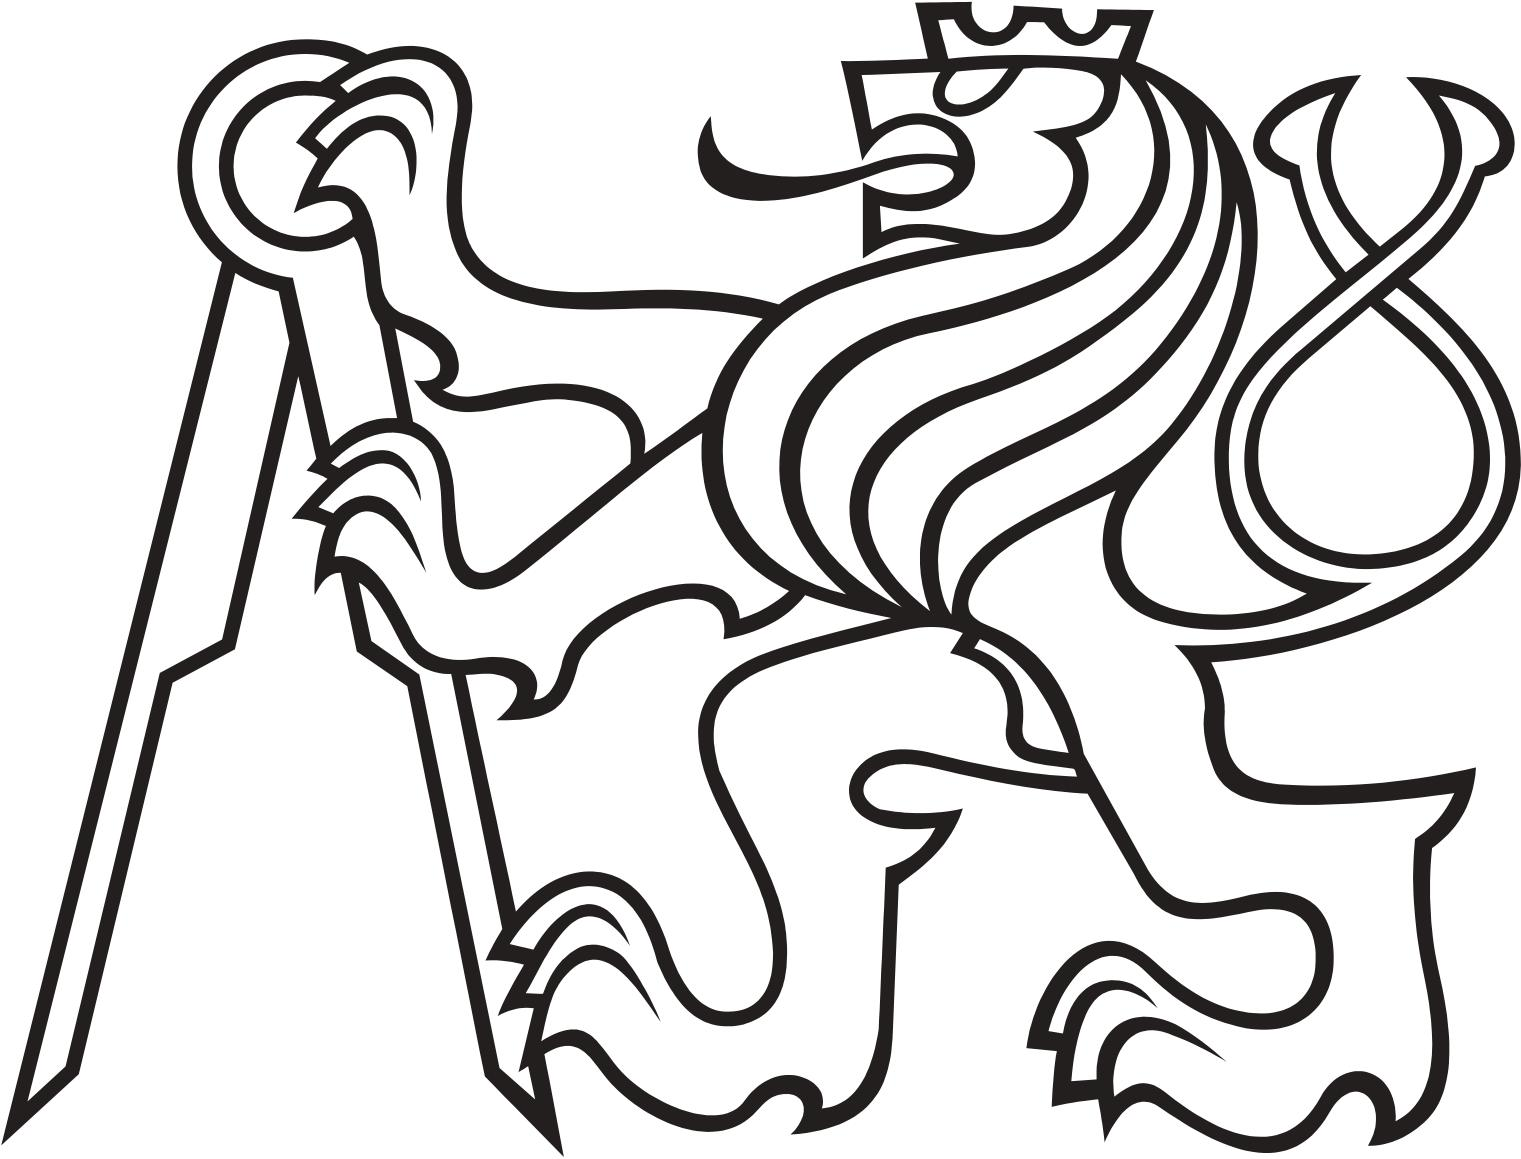
\includegraphics[width=0.3\textwidth]{src/ctu_logo_black.jpg}

%========== Date ==========
\vfill\vfill
{\large\monthyeardate\today}
% Push the date up 1/4 of the remaining page
\vfill
\end{titlepage}

%========== Blank page ==========
\newpage\blankpage

% %========== Assignment ==========
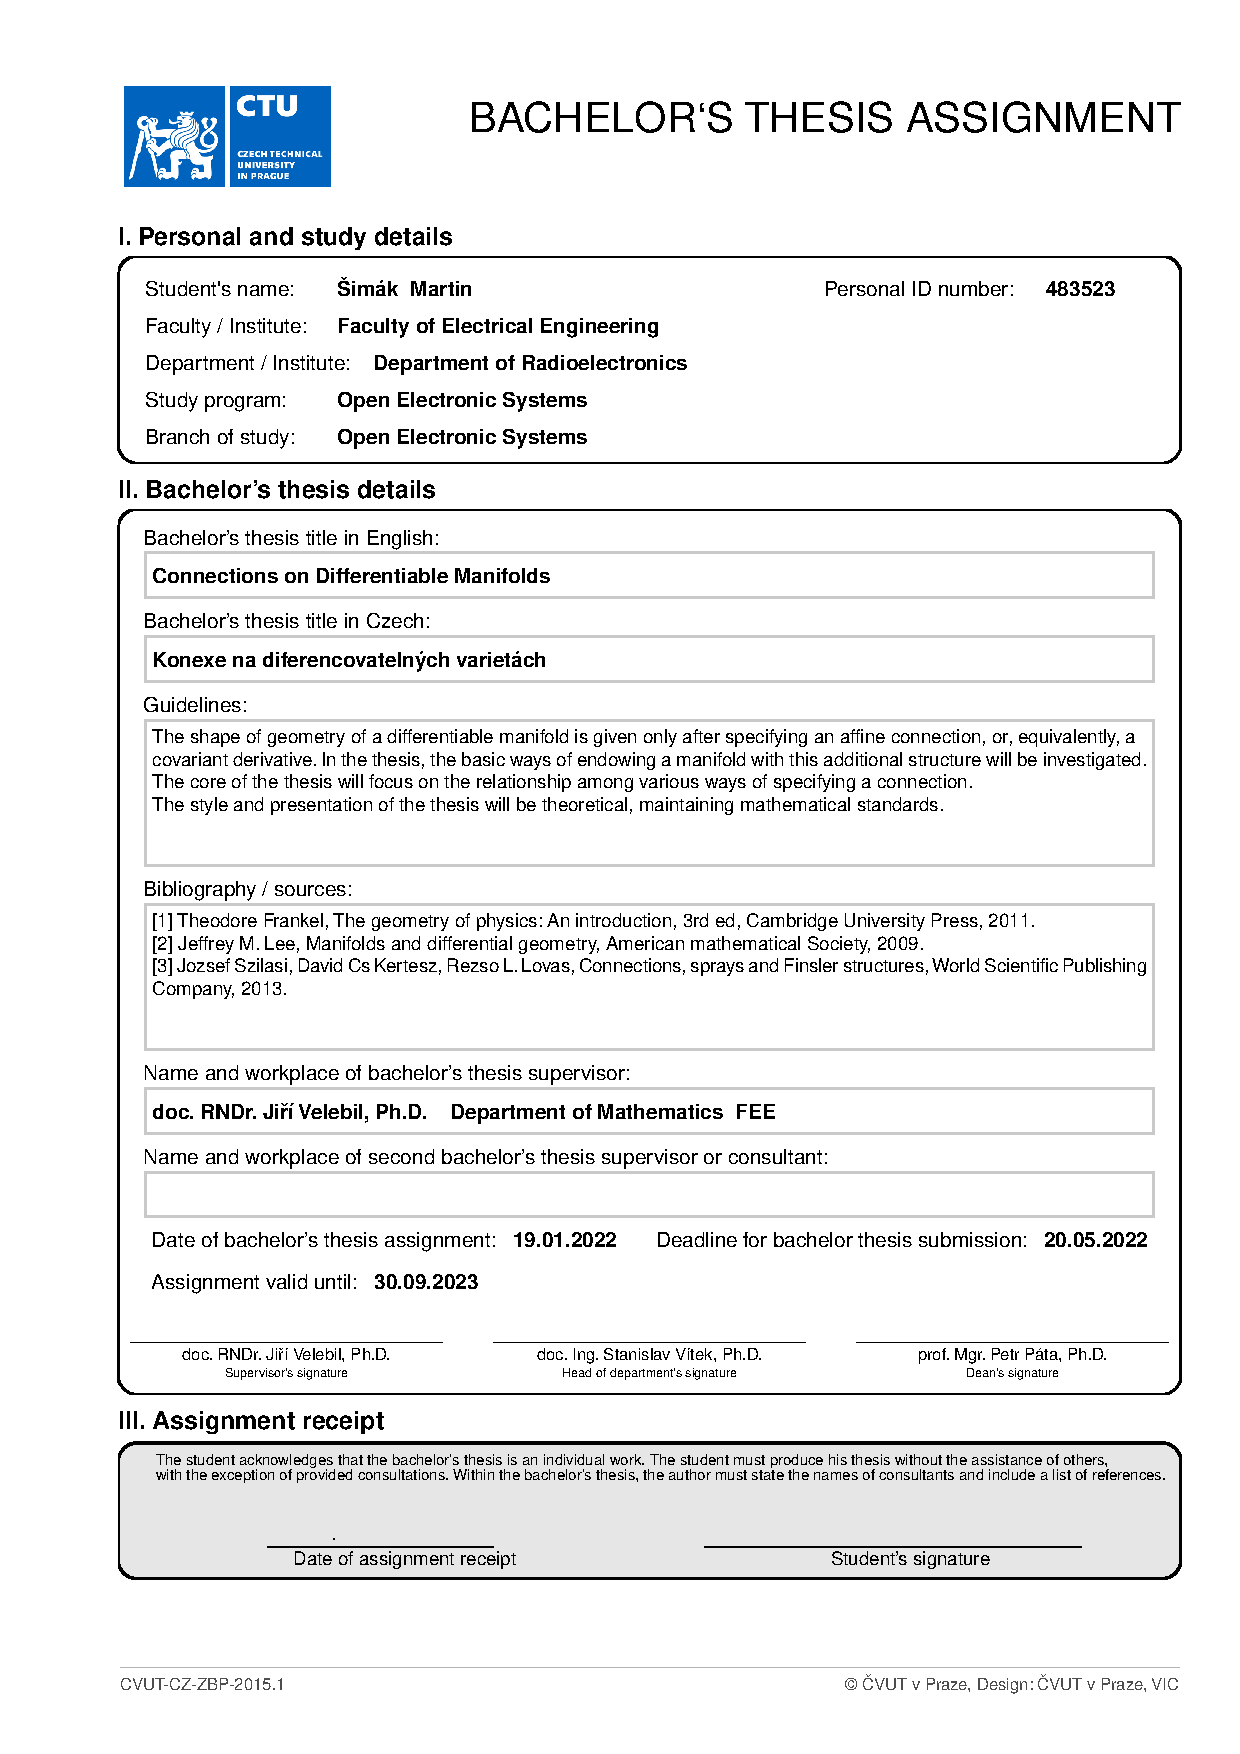
\includepdf[pages=-]{src/assignment.pdf}

% Start counting pages in roman numerals
\pagenumbering{roman}

% %========== Declaration ==========
% \clearpage
\vspace*{\fill}
\noindent\textbf{Declaration}\\[0.25cm]
I declare that I completed the presented thesis independently and that all used sources are quoted in accordance with the Methodological instructions that cover the ethical principles for writing an academic thesis.\\
\hrule\vspace*{1cm}
\begin{otherlanguage}{czech}
    \noindent\textbf{Prohlášení}\\[0.25cm]
    Prohlašuji, že jsem předloženou práci vypracoval samostatně a že jsem uvedl veškeré použité informační zdroje v souladu s Metodickým pokynem o dodržování etických principů při přípravě vysokoškolských závěrečných prací.\\
    \begin{center}
        \begin{minipage}{0.45\textwidth}
            \begin{flushleft}
                V Praze \hdashrule{3cm}{0.5pt}{2pt}
            \end{flushleft}
        \end{minipage}
        ~
        \begin{minipage}{0.45\textwidth}
            \begin{flushright}
                \noindent\begin{tabular}{c}
                    \\
                    \hdashrule{4cm}{0.5pt}{2pt}\\
                    Martin Šimák
                \end{tabular}
            \end{flushright}
        \end{minipage}
    \end{center}
\end{otherlanguage}
\clearpage

% %========== Acknowledgements ==========
% \clearpage
\vspace*{\fill}
\noindent\textbf{Acknowledgements}\\[0.25cm]
Above all, I would like to thank my supervisor, doc. Ing. Pavel Hazdra, Ph.D., for his professional help, willingness, and reliable correspondence throughout our collaboration, which took place remotely during my double degree program in cooperation with the National Taiwan University of Science and Technology. I would also like to thank my supervisor, Ding-Bing Lin, who is responsible for the content of this thesis at the partner university, for his initiative and valuable assistance, especially in the design production. Last but not least, I would like to thank all my loved ones who supported me from afar throughout my studies, especially my family and friends. Special thanks go to Ester \foreignlanguage{czech}{Jančaříková} for standing by me and helping me through difficult times.\\
\hrule\vspace*{1cm}
\begin{otherlanguage}{czech}
    \noindent\textbf{Poděkování}\\[0.25cm]
    Především bych rád poděkoval svému vedoucímu, doc. Ing. Pavlu Hazdrovi, Ph.D., za jeho odbornou pomoc, vstřícnost, a ochotu v podobě spolehlivé korespondence během spolupráce, která probíhala distančně v rámci mého studia double degree programu ve spolupráci s National Taiwan University of Science and Technology. Dále děkuji svému vedoucímu Ding-Bing Linovi, který odpovídá za náplň této práce na partnerské univerzitě, za jeho iniciativu a cennou pomoc, zejména při výrobě návrhu. V neposlední řadě bych rád poděkoval všem svým blízkým, kteří mě na dálku podporovali během celého studia, zejména své rodině a přátelům. Zvláštní poděkování na závěr potom patří Ester Jančaříkové za to, že stála při mě a byla mi oporou v nelehkých chvílích.
\end{otherlanguage}
\clearpage

% %========== Abstract ==========
% \clearpage
\noindent\textit{Title:}\\
\textbf{Dual Circularly Polarized Waveguide Antenna}\\[0.25cm]
\textit{Author:} Martin Šimák\\[0.25cm]
\textit{Study programme:} Electronics and Communications\\[0.25cm]
\textit{Supervisor:} doc. Ing. Pavel Hazdra, Ph.D., Department of Electromagnetic Field FEE\\[0.25cm]
\textit{Abstract:}\\
This thesis details the design, simulation, fabrication, and measurement of a novel dual circularly polarized antenna operating in the $\frequencyrange$ band. The system comprises a square waveguide polarizer with chamfered corners, a dual-coaxial feed, and a conical horn antenna. The polarizer generates right-hand and left-hand circular polarization by selectively exciting one of the two fundamental modes of the square waveguide. The dual coaxial feed provides the necessary excitation. The conical horn, designed using Antenna Magus and adapted to the polarizer, achieves a target gain of $\qty{15}{dBi}$. CST Studio Suite was used for electromagnetic simulations, while Python with SciPy enabled dynamic optimization for enforcing geometric constraints. The fabricated antenna's measured performance closely aligns with simulations, demonstrating an axial ratio below $\qty{5}{dB}$ across the band and a measured gain of approximately $\qty{18}{dBi}$ at the centre frequency. This work contributes to a compact, manufacturable, dual circularly polarized antenna design with potential applications in satellite communications, radar, and other wireless systems.\\[0.25cm]
\textit{Keywords:} circular polarization, waveguide polarizer, dual-feed, conical horn antenna, hexagonal waveguide, eigenmode analysis, electromagnetic simulation\\[0.5cm]
\begin{otherlanguage}{czech}
    \noindent\textit{Název práce:}\\
    \textbf{Duálně kruhově polarizovaná vlnovodová anténa}\\[0.25cm]
    \textit{Autor:} Martin Šimák\\[0.25cm]
    \textit{Studijní program:} Elektronika a komunikace\\[0.25cm]
    \textit{Vedoucí:} doc. Ing. Pavel Hazdra, Ph.D., Katedra elektromagnetického pole FEL\\[0.25cm]
    \textit{Abstrakt:}\\
    Tato diplomová práce popisuje návrh, simulaci, výrobu a měření duální kruhově polarizované antény pracující v pásmu $\frekvencnipasmo$. Systém se skládá ze čtvercového vlnovodného polarizátoru se zkosenými rohy, dvojitého koaxiálního napájení a kuželové antény. Polarizátor generuje pravotočivou a levotočivou kruhovou polarizaci selektivně buzené jedním ze dvou základních módů čtvercového vlnovodu. Potřebné buzení zajišťuje duální koaxiální napájení. Kuželová anténa navržená pomocí programu Antenna Magus a přizpůsobená polarizátoru dosahuje cílového zisku $\qty{15}{dBi}$. Pro elektromagnetické simulace byla použit software CST Studio Suite, zatímco Python s použitím knihovny SciPy umožnil dynamickou optimalizaci pro vynucení geometrických omezení. Naměřený výkon zhotovené antény se přesně shoduje se simulacemi a vykazuje osový poměr pod $\qty{5}{dBi}$ v celém pásmu a naměřený zisk přibližně $\qty{18}{dBi}$ na střední frekvenci. Tato práce přináší kompaktní, vyrobitelnou konstrukci duální kruhově polarizované antény s potenciálním využitím v satelitní komunikaci, radarové technice a dalších bezdrátových systémech.\\[0.25cm]
    \textit{Klíčová slova:} kruhová polarizace, vlnovodný polarizátor, duální napájení, kuželová anténa, hexagonální vlnovod, analýza vlastních módů, elektromagnetická simulace\\[0.5cm]
\end{otherlanguage}
\clearpage

% Start counting pages in arabic numerals
\pagenumbering{arabic}

%========== Table of contents ==========
\tableofcontents

%========== Introduction ==========
\chapter*{Introduction}
\label{chap:introduction}
\addcontentsline{toc}{chapter}{\nameref{chap:introduction}}

Do not write a couple of words on literature survey. Present the difference construction and design choices, compare them both theoretically and by the results presented in gathered papers, but in their respective sections of the design process. Use them a nice foreword for each of the parts, going through existing approaches.

\lipsum[1]

Throughout the theoretical chapter, I omit using the common \emph{del}, or \emph{nabla}, notation for the vector differential operator $\nabla$ which gives rise to the formally proper differential operators of gradient ($\nabla$), divergence ($\nabla\cdot$), curl ($\nabla\times$), and sometimes even the Laplace operator ($\nabla\cdot\nabla$ or $\nabla^2$). Instead, I will use the standard notations of $\Grad$, $\Div$, $\Curl$, and $\Delta$, respectively. While I am aware of the mnemonic merits it brings when working in coordinates, this does not come to fruition as I do not carry out any computations in this text. On the other hand, there are various reasons to avoid it, such as that it promotes a notational ambiguity with the covariant derivative used in differential geometry, or to distinguish the individual operators at first sight better.
\nomenclature{$\Grad$}{gradient }%
\nomenclature{$\Div$}{divergence }%
\nomenclature{$\Curl$}{curl }%
\nomenclature{$\Delta$}{Laplace operator }%

\paragraph*{Synopsis.} In \textbf{\cref{chap:electrodynamics}}, \lipsum[4]

\paragraph*{Methodology.} \lipsum[4]


%========== Chapter 1: Electrodynamics of guided waves ==========
\chapter{Electrodynamics of guided waves}
\label{chap:electrodynamics}
This chapter establishes the theoretical foundation for the analysis and design of a waveguide-based antenna system. Beginning with Maxwell's equations and general description of electromagnetic fields in various settings relevant to this work, the wave equations governing guided modes are derived, and their solutions are analysed to elucidate the behaviour of electromagnetic fields within waveguides. This analysis provides a framework for understanding the operation of structures designed in the following chapters. While focusing on the essential elements of waveguide theory, this chapter provides a comprehensive treatment of the subject and establishes the notation used throughout this work.

The exposition endeavours to build upon the foundations laid in \parencite{balanis:advanced-engineering-electromagnetics,griffiths:introduction-to-electrodynamics}, incorporating personal insights and notational preferences to present a cohesive foundation for further chapters.

\section{Fundamentals of electrodynamics}
\label{sec:fundamentals-of-electrodynamics}
In this section, the fundamental principles of electromagnetism are presented, starting with Maxwell's equations, which encapsulate the relationships between electric and magnetic fields and their sources. The response of different materials to these fields is then explored through the introduction of \emph{constitutive relations}. Finally, the focus is shifted to the behaviour of electromagnetic fields at material boundaries, providing essential \emph{boundary conditions} for solving electromagnetic problems.

\subsection{Maxwell's equations}
The differential form of Maxwell's equations, as presented below, constitutes the cornerstone of classical electromagnetism, providing a complete%
    \footnote{For actual completeness (save for some special properties stemming from interactions in matter), the equations must also be supplemented by the Lorentz's force law $\vec F = q(\vec E + \vec v \times \vec B)$.}
framework for analysing electromagnetic phenomena at any point in space and time. These equations summarize the relations between \emph{electric field intensity}~$\vec E$ and \emph{magnetic flux density}~$\vec B$ and their sources due to charge densities~$\rho$, current densities~$\vec J$, or the changing of the fields themselves. To ensure the validity of these expressions, let us assume that the field vectors are well-behaved functions, exhibiting continuity and possessing continuous derivatives. This assumption holds for most electromagnetic systems, with exceptions arising at interfaces between distinct media where abrupt changes in charge and current densities may occur.

\begin{subequations}
    \label[pluralequation]{subeq:maxwell-general}
    \noindent\centering
    \begin{minipage}{0.45\textwidth}
        \begin{align}
            \label{eq:maxwell-general-div-e}
            \Div\vec E &= \frac1{\epsilon_0}\rho_{\mathrm e},
        \\
            \label{eq:maxwell-general-curl-e}
            \Curl\vec E &= -\mu_0\vec J_{\mathrm m} - \partial_t\vec B,
        \end{align}
    \end{minipage}
    \hfill
    \begin{minipage}{0.45\textwidth}
        \begin{align}
            \label{eq:maxwell-general-div-b}
            \Div\vec B &= \mu_0\rho_{\mathrm m},\vphantom{\frac1{\epsilon_0}}
        \\
            \label{eq:maxwell-general-curl-b}
            \Curl\vec B &= \mu_0\vec J_{\mathrm e} + \mu_0\epsilon_0\partial_t\vec E,
        \end{align}
    \end{minipage}
    \nomenclature{$\partial_\xi$}{partial derivative w.r.t. variable $\xi$ }%
    \nomenclature{$\vec E$}{electric field intensity }%
    \nomenclature{$\vec B$}{magnetic flux density }%
    \nomenclature{$\rho_{\mathrm e}$}{electric charge density }%
    \nomenclature{$\rho_{\mathrm m}$}{magnetic charge density }%
    \nomenclature{$\vec J_{\mathrm e}$}{source electric current density }%
    \nomenclature{$\vec J_{\mathrm m}$}{magnetic current density }%
    \bigskip
\end{subequations}

There is one oddity about \cref{subeq:maxwell-general} and that is the inclusion of the magnetic charge density $\rho_{\mathrm m}$ and magnetic current density $\vec J_{\mathrm m}$ which are part of the \enquote{generalized concept}. Although these quantities, in spite of diligent search, were never physically observed, their introduction establishes a pleasing balance in Maxwell's equations while being theoretically sound as well. This concept is further utilized when solving advanced physical problems in applied physics and engineering. This is facilitated by the introduction of equivalent magnetic charge and current which can be used to conveniently express fields as if generated by these fictitious sources, especially in problems where the exact form of the electromagnetic field would otherwise be complicated to elucidate.

Mathematically, \cref{subeq:maxwell-general}, like any differential equations, form a complete problem only when supplemented with suitable boundary conditions in a more traditional sense, such as behaviour of the vector fields \enquote{in infinity}. These are typically \enquote{obvious} from the problem-solving context, e.g., fields vanishing at large distance from localized charge distribution, etc.

\subsection{Electromagnetic properties of matter}
Although Maxwell's equations in their fundamental form \eqref{subeq:maxwell-general} provide a complete description of electromagnetic phenomena, an alternative formulation offers a more convenient approach for analysing materials susceptible to electric and magnetic polarization. Within such media, the total electric charge density~$\rho_{\mathrm e}$ can be expressed as a sum of the \emph{free charge} density~$\rho_{\mathrm f}$, which constitutes the \emph{actual source} charge,%
    \footnote{It is important to reinforce the idea that the magnetic charge and current are fictitious \enquote{source} quantities. Therefore, they are already, by definition, purely \emph{free} quantities.}
and the \emph{bound charge}~$\rho_{\mathrm b}=-\Div\vec P$, produced by an electric polarization~$\vec P$ of the material. Moreover, changing electric fields also induce changing polarization, producing \emph{polarization current}~$\vec J_{\mathrm p}=\partial_t\vec P$ which add to the \emph{free current}~$\vec J_{\mathrm f}$. Similarly to electric polarization, a magnetic polarization~$\vec M$ results in a bound current~$\vec J_{\mathrm b}=\Curl\vec M$. These effects, inherently connected to the susceptibility of materials to be polarized, hence influence the total electromagnetic field in their vicinity. This led to the introduction of convenient field quantities that account for the presence of such media.

Within the framework of Maxwell's equations, \emph{electric flux density}~$\vec D$ (also called the \emph{electric displacement field}) and the \emph{magnetic field intensity}~$\vec H$ offer a more convenient representation, explicitly separating the free and bound sources. This approach allows for expressing Maxwell's equations in a form that directly relates the fields to the free charge and free current, which are sources that can be controlled directly. Using these field quantities, \cref{subeq:maxwell-general} read

\begin{subequations}
    \label[pluralequation]{subeq:maxwell-general-matter}
    \noindent\centering
    \begin{minipage}{0.45\textwidth}
        \begin{align}
            \label{eq:maxwell-general-matter-div-d}
            \Div\vec D &= \rho_{\mathrm f},
        \\
            \label{eq:maxwell-general-matter-curl-e}
            \Curl\vec E &= -\vec J_{\mathrm m} - \partial_t\vec B,
        \end{align}
    \end{minipage}
    \hfill
    \begin{minipage}{0.45\textwidth}
        \begin{align}
            \label{eq:maxwell-general-matter-div-b}
            \Div\vec B &= \mu_0\rho_{\mathrm{m}},
        \\
            \label{eq:maxwell-general-matter-curl-h}
            \Curl\vec H &= \vec J_{\mathrm f} + \partial_t\vec D,
        \end{align}
    \end{minipage}
    \nomenclature{$\vec D$}{electric flux density }%
    \nomenclature{$\vec H$}{magnetic field intensity }%
    \bigskip
\end{subequations}

While \cref{subeq:maxwell-general-matter} effectively express electromagnetic laws within media, their hybrid notation, involving both $\vec E$ and $\vec D$, and both $\vec B$ and $\vec H$, necessitates the use of \emph{constitutive relations}. These relations, which establish correspondence between the respective electric and magnetic field quantities, are material-dependent and reflect the specific response of a medium to electric and magnetic fields. In general, these relationships can be expressed as
\begin{subequations}
    \index{constitutive relations}
    \index{constitutive parameters}
    \label[pluralequation]{subeq:constitutive-relations}
    \begin{align}
        \label{eq:constitutive-relation-permittivity}
        \vec D &= \hat\epsilon \ast \vec E,
    \\
        \label{eq:constitutive-relation-permeability}
        \vec B &= \hat\mu \ast \vec H,
    \end{align}
    \nomenclature{$\epsilon$}{permittivity }%
    \nomenclature{$\mu$}{permeability }%
\end{subequations}
where $\hat\epsilon$ and $\hat\mu$ are the material's \emph{permittivity} and \emph{permeability}, respectively, and the asterisk denotes \emph{convolution}.

\begin{remark}
    In formulations of akin to \cref{subeq:maxwell-general-matter}, with emphasis on the separation of free and bound sources, some authors prefer to further dissect the free current, too. This current is generally conceptualized as the current \enquote{not directly tied to the bound charges} within a material. To name a few commonly recognized, \emph{convection current}, \emph{beam current}, or \emph{conduction current}. It is the conduction current which is, in electrical engineering, especially worth mentioning because it arises from the movement of charges, typically electrons, that can move freely throughout the material. This kinetic energy of charges in conductors is the main cause of losses in waveguides and can be expressed by
    \begin{align}
        \label{eq:constitutive-relation-conductivity}
        \vec J_{\mathrm c} &= \hat\sigma \ast \vec E,
        \nomenclature{$\sigma$}{conductivity }%
    \end{align}
    where $\hat\sigma$ is the material's \emph{conductivity}. \Cref{eq:constitutive-relation-conductivity}, together with \cref{subeq:constitutive-relations}, completes the required set of constitutive relations.
\end{remark}

The \emph{constitutive parameters} $\hat\epsilon$, $\hat\mu$, and $\hat\sigma$, generally represented as complex second-rank tensors, establish the relationship between the applied electromagnetic fields and the material's response. The functional dependencies of these tensors provide a classification scheme for material properties:
\begin{itemize}
    \item \emph{Linearity:} A material is classified as linear if its constitutive parameters are independent of the applied field strength; otherwise, it is considered nonlinear.
    \item \emph{Homogeneity:} If the constitutive parameters are invariant with respect to position within the material, it is deemed homogeneous; conversely, spatial dependence indicates an inhomogeneous medium.
    \item \emph{Isotropy:} Materials exhibiting constitutive parameters independent of the applied field's direction are classified as isotropic. Conversely, direction-dependent parameters signify an anisotropic material, with crystals being a prime example.
    \item \emph{Dispersion:} Materials whose constitutive parameters exhibit frequency dependence are categorized as dispersive. While some materials demonstrate negligible frequency dependence and can be effectively considered nondispersive, all materials encountered in practice exhibit some degree of dispersion.
\end{itemize}

\begin{example}[Constitutive relations in free space]
    In the simplest case of free space, equations~\eqref{eq:constitutive-relation-permittivity},~\eqref{eq:constitutive-relation-permeability},~and~\eqref{eq:constitutive-relation-conductivity} become
    \begin{subequations}
        \begin{align}
            \hat\epsilon &= \epsilon_0 \approx 8.854\times 10^{-12}\ \unit{F.m^{-1}},
        \\
            \hat\mu &= \mu_0 = 4\pi\times 10^{-7}\ \unit{H.m^{-1}},
        \\
            \hat\sigma &= \sigma_0 = 0\ \unit{S.m^{-1}}.
        \end{align}
    \end{subequations}
\end{example}

\subsection{Boundary conditions}
While the differential forms of Maxwell's equations are powerful tools for analysing electromagnetic fields within continuous media, material boundaries introduce discontinuities that require special treatment. These discontinuities in the fields $E$, $B$, $D$, and $H$ arise at interfaces between media with different electrical properties or at surfaces carrying charge or current densities. To accurately describe the behaviour of the fields across such boundaries, Maxwell's equations in their integral form, which naturally incorporate these discontinuities, are more convenient. This form is obtained by applying integral theorems from vector calculus to \cref{subeq:maxwell-general-matter} which then take on the form of\\
\begin{subequations}
    \index{boundary conditions}
    \label[pluralequation]{subeq:maxwell-equations-integral}
    \noindent\centering
    \begin{align}
        \label{eq:maxwell-equations-integral-div-d}
        \oint_S \vec D \cdot \d\vec a &= Q_{\mathrm{e}},
    \\
        \label{eq:maxwell-equations-integral-curl-e}
        \oint_{\partial S} \vec E \cdot \d\vec l &= -\int_S \vec J_{\mathrm m} \cdot \d\vec a - \frac{\d}{\d t}\int_S \vec B \cdot \d\vec a,
    \\
        \label{eq:maxwell-equations-integral-div-b}
        \oint_S \vec B \cdot \d\vec a &= Q_{\mathrm{m}},
    \\
        \label{eq:maxwell-equations-integral-curl-h}
        \oint_{\partial S} \vec H \cdot \d\vec l &= \int_S \vec J_{\mathrm e} \cdot \d\vec a + \frac{\d}{\d t}\int_S \vec D \cdot \d\vec a.
    \end{align}
    \nomenclature{$\partial\Omega$}{boundary of set $\Omega$ }%
\end{subequations}\\
where $S$ is any closed surface.

Consider a boundary between two different media. The first medium is characterized by permittivity $\epsilon_1$ and permeability $\mu_1$, while the second medium is characterized by permittivity $\epsilon_2$ and permeability $\mu_2$. At this interface, electric and magnetic surface charge densities, denoted by $q_f$ and $q_m$ respectively, may be present. Additionally, electric and magnetic surface current densities, denoted by $j_f$ and $j_m$ respectively, may also exist. The general \emph{boundary conditions} for electrodynamics are then obtained by applying equations \cref{subeq:maxwell-equations-integral} to arbitrary surfaces encompassing a portion of the interface, yielding

\begin{subequations}
    \label[pluralequation]{subeq:boundary-conditions}
    \noindent\centering
    \begin{minipage}{0.45\textwidth}
        \begin{align}
            \label{eq:boundary-conditions-d-normal}
            \vec e_n \cdot (\vec D_1 - \vec D_2) &= q_{\mathrm f},
        \\
            \label{eq:boundary-conditions-e-tangential}
            -\vec e_n \times (\vec E_1 - \vec E_2) &= \vec j_{\mathrm m},
        \end{align}
    \end{minipage}
    \hfill
    \begin{minipage}{0.45\textwidth}
        \begin{align}
            \label{eq:boundary-conditions-b-normal}
            \vec e_n \cdot (\vec B_1 - \vec B_2) &= q_{\mathrm m},
        \\
            \label{eq:boundary-conditions-H-tangential}
            \vec e_n \times (\vec H_1 - \vec H_2) &= \vec j_{\mathrm f}.
        \end{align}
    \end{minipage}
    \bigskip
\end{subequations}

\section{Electromagnetic waves}
\label{sec:electromagnetic-waves}
Having established the foundations of electromagnetism, the focus is now shifted to one of its most significant consequences: the existence of electromagnetic waves. In this section, the manner in which Maxwell's equations predict the propagation of these waves is explored.  The wave equations for the electric and magnetic fields are derived, revealing their interconnected nature and their ability to sustain each other even in the absence of sources. Subsequently, the simplest and most fundamental solutions to these equations, \emph{monochromatic plane waves}, are investigated. Finally, the confinement and guidance of these plane waves within conducting cavities is examined, laying the groundwork for understanding waveguides and resonant structures.

\subsection{The wave equations}
Maxwell's equations provide a comprehensive description of electromagnetic phenomena, but their coupled nature can make them challenging to solve directly. To facilitate analysis, particularly in source-free regions, it's often advantageous to decouple the equations and express them in terms of the electric and magnetic fields individually. Inside regions with no \emph{free} charge or \emph{free} current, Maxwell's \cref{subeq:maxwell-general-matter} take on the form of\\
\begin{subequations}
    \label[pluralequation]{subeq:maxwell-sourceless}
    \noindent\centering
    \begin{minipage}{0.45\textwidth}
        \begin{align}
            \label{eq:maxwell-sourceless-div-d}
            \Div \vec D &= 0,
        \\
            \label{eq:maxwell-sourceless-curl-e}
            \Curl \vec E &= -\partial_t\vec B,
        \end{align}
    \end{minipage}
    \hfill
    \begin{minipage}{0.45\textwidth}
        \begin{align}
            \label{eq:maxwell-sourceless-div-b}
            \Div\vec B &= 0,
        \\
            \label{eq:maxwell-sourceless-curl-h}
            \Curl\vec H &= \sigma\vec E + \partial_t\vec D.
        \end{align}
    \end{minipage}\bigskip
\end{subequations}\\
Furthermore, if the medium is \emph{linear} and \emph{homogeneous}, \cref{eq:maxwell-sourceless-curl-h} can be fully expressed in terms of $\vec E$. With this simplification, applying the curl to \cref{eq:maxwell-sourceless-curl-e,eq:maxwell-sourceless-curl-h} yields

\begin{subequations}
    \label[pluralequation]{subeq:wave-equations-lossy}
    \noindent\centering
    \begin{minipage}{0.45\textwidth}
        \begin{align}
            \label{eq:wave-equation-e}
            \Delta\vec E &= \mu\sigma\partial_t\vec E + \mu\epsilon\partial^2_t\vec E,
        \end{align}
    \end{minipage}
    \hfill
    \begin{minipage}{0.45\textwidth}
        \begin{align}
            \label{eq:wave-equation-b}
            \Delta\vec B &= \mu\sigma\partial_t\vec B + \mu\epsilon\partial^2_t\vec B.
        \end{align}
    \end{minipage}\bigskip
\end{subequations}

Therefore, electric and magnetic fields in linear homogeneous media both clearly satisfy the wave equation with a linear damping term $\mu\sigma\partial_t$, introduced by conductive losses. Moreover, in regions with $\sigma = 0$, such as free space or ideal insulators, \cref{subeq:wave-equations-lossy} simplify even more to\\
\begin{subequations}
    \label[pluralequation]{subeq:wave-equations-lossless}
    \noindent\centering
    \begin{minipage}{0.45\textwidth}
        \begin{align}
            \label{eq:wave-equation-e-lossless}
            \Delta\vec E &= \mu\epsilon\partial^2_t\vec E,
        \end{align}
    \end{minipage}
    \hfill
    \begin{minipage}{0.45\textwidth}
        \begin{align}
            \label{eq:wave-equations-b-lossless}
            \Delta\vec B &= \mu\epsilon\partial^2_t\vec B,
        \end{align}
    \end{minipage}\bigskip
\end{subequations}\\
taking on the form of classical wave equations which are ubiquitous in physics. This also immediately gives rise to the formula
\begin{align}
    v &= \frac{1}{\sqrt{\epsilon\mu}} = \frac{c}{\sqrt{\epsilon_r\mu_r}}
\end{align}
for the speed of electromagnetic waves in linear homogeneous media.

\begin{remark}
    \label{remark:nonequivalence-of-wave-equations-with-maxwells-equations}
    Compared with the original Maxwell's \cref{subeq:maxwell-general-matter}, these equations form two systems of partial differential equations of second order but are now decoupled and provide us with an additional solving method for given boundary-value problems. However, it is important to note that the wave \cref{eq:wave-equation-e,eq:wave-equation-b} were derived from Maxwell's \cref{subeq:maxwell-sourceless} by differentiation. This impedes their mathematical equivalence. More specifically (as stated in~\parencite{griffiths:introduction-to-electrodynamics}), whereas every solution to Maxwell's equations is also a solution for the wave equations, the converse is not true.
\end{remark}

\subsection{Monochromatic plane waves}
\index{monochromatic plane wave}
The electromagnetic theory presented thus far describes general vector fields that vary in space and time. However, as shown in \cref{sec:electromagnetic-waves}, electromagnetic fields in source-free regions exhibit wave behaviour. Nonetheless, these time-varying vector fields remain complex and challenging to analyse in practical systems. Consider the elementary solution to the wave equation
\begin{align}
    \label{eq:monochromatic-plane-wave}
    \hat{\vec\psi}(\vec r,t) &= \hat{\vec\Psi}_0\exp\[\i\(\hat{\vec k} \cdot \vec r-\omega t\)\].
\end{align}
\nomenclature{$\vec k$}{wave vector }%
Here, $\hat{\vec k}$ is the complex \emph{wave vector} indicating the direction of wave propagation, and $\omega$ is the angular frequency of the wave. \Cref{eq:monochromatic-plane-wave} is expressed in terms of a \emph{complex wave function} with a \emph{complex amplitude} $\hat{\vec\Psi}_0 \equiv \vec\Psi_0\e^{\i\varphi}$. This quantity encapsulates both the \emph{real amplitude} $\vec\Phi_0$ and the \emph{phase shift} $\varphi$, of the physical wave. A sinusoidal wave representing this solution in physical reality can be extracted from \cref{eq:monochromatic-plane-wave} using the \emph{Euler's formula}, yielding
\begin{align}
    \label{eq:sinusoidal-wave}
    \vec{\psi}(\vec r, t) &= \Re\[\hat{\vec\Psi}_0\exp\[\i\(\hat{\vec k} \cdot \vec r-\omega t+\varphi\)\]\] = \Re\[\hat{\vec\psi}(\vec r, t)\].
\end{align}

\begin{remark}
    Clearly, if \cref{eq:sinusoidal-wave} satisfies \cref{subeq:wave-equations-lossless} and Maxwell's equations, the same holds true for \cref{eq:monochromatic-plane-wave}, as the imaginary part differs from the real part only by the replacement of sine with cosine.
\end{remark}

\Cref{eq:monochromatic-plane-wave} serves as as an established elementary solution to the general wave equation, and hence also to \cref{subeq:wave-equations-lossless}. Substituting this solution into \cref{subeq:wave-equations-lossy}, it becomes evident that these \enquote{lossy wave equations} also admit plane-wave solutions. Furthermore, this substitution allows for the derivation of a general formula for the complex \emph{wavenumber}
\begin{align}
    \label{eq:wave-number}
    \hat k^2 = \hat{\vec k} \cdot \hat{\vec k} = \mu\epsilon\omega^2 + \i\mu\sigma\omega.
\end{align}
In the context of \cref{eq:monochromatic-plane-wave}, it is evident that the real part of the complex wavenumber $\hat k$ is the \emph{actual} wavenumber as it determines the change of phase with spatial propagation. For this reason, the real part is simply denoted $k$ and is called the \emph{phase constant}. In contrast, the imaginary part of $\hat k$ is responsible for the exponential damping, or attenuation, in conductive media, and hence is called the \emph{attenuation constant}.

Waves described by \cref{eq:monochromatic-plane-wave} are called \emph{monochromatic}, or \emph{time-harmonic}, \emph{plane}
waves. Monochromaticity refers to the fact that the wave oscillates at a single frequency $\omega$ through time, while planarity indicates that the fields are uniform over every plane perpendicular to the direction of propagation. Although less common, plane waves could alternatively be called \emph{space-harmonic},%
    \footnote{Therefore, monochromatic plane waves are something one could call \emph{spacetime-harmonic} or simply \emph{harmonic}.}
as both of these terms signify a sinusoidal dependence on a given variable. In the case of monochromaticity, the variable is time, oscillating with an angular frequency $\omega$. Similarly, planarity reflects the waveform repetition in the spatial coordinates, projected into the propagation direction, with a well-defined spatial frequency $k$.

The significance of this particular solution stems from the fact that, in practice, any wave we will be dealing with can be expressed as a linear combination of these monochromatic plane waves, i.e.,
\begin{align}
    \label{eq:fourier-transform}
    \hat{\vec\psi}(\vec r,t) &= \int_{\R^3} \hat{\vec{\Psi}}_0(\vec k)\exp\[\i\(\hat{\vec k} \cdot \vec r-\omega t\)\]\, \d\vec k.
\end{align}
This superposition principle mathematically reflects the Fourier transform over every plane wave corresponding to a given frequency $\omega$. With this formally sound mathematical description, the existence of a unique linear combination for \enquote{any wave we will be dealing with}, as vaguely stated above, can be rigorously established through the following theorem.
\begin{theorem}[Dirichlet-Jordan test]
    \label{theorem:dirichlet-jordan-test}
    Let $f$ be a function in $L^1(-\infty,\infty)$ and of bounded variation in a neighbourhood of the point $x$. Then
    \begin{align}
        \frac1\pi \lim_{M\to\infty}\int_0^M\,\d u \int_\R f(t)\cos(u(x-t))\,\d t = \lim_{\epsilon\to0}\frac{f(x+\epsilon)+f(x-\epsilon)}2.
    \end{align}
    If $f$ is continuous in an open interval, then the integral on the left-hand side converges uniformly in the interval, and the limit on the right-hand side is $f(x)$.
\end{theorem}
More details on this mathematical theory can be found in~\parencite{titchmarsh:introduction-to-the-theory-of-fourier-integrals}. A version of \cref{theorem:dirichlet-jordan-test}, retaining the original form due to Dirichlet, is often used in signal processing. More details on that formulation can be found, e.g., in~\parencite{oppenheim:signals-and-systems}.

Since any physically realizable signal is square-integrable and has compact support,%
    \footnote{In the field of signal processing, these signal properties are often described as having \emph{finite energy} and \emph{duration}, respectively.}
this text's attention is confined to monochromatic plane waves. Therefore, the fields take on the form of\\
\begin{subequations}
    \label[pluralequation]{subeq:monochromatic-plane-wave-fields}
    \begin{align}
        \label{eq:monochromatic-plane-wave-e}
        \hat{\vec E}(\vec r, t) &= \hat{\vec E}_0 \exp\[\i\(\hat{\vec k} \cdot \vec r-\omega t\)\],
    \\
        \label{eq:monochromatic-plane-wave-b}
        \hat{\vec B}(\vec r, t) &= \hat{\vec B}_0 \exp\[\i\(\hat{\vec k} \cdot \vec r-\omega t\)\],
    \end{align}
\end{subequations}
where $\hat{\vec E}_0$ and $\hat{\vec B}_0$ are complex amplitudes.

As discussed in \cref{remark:nonequivalence-of-wave-equations-with-maxwells-equations}, satisfying the wave equations does not guarantee solutions to Maxwell's equations. Substituting the solutions of the wave equations into Maxwell's equations is necessary, as it might refine the solutions or yield more information. As an example, consider the plane waves in vacuum.

\begin{example}[Monochromatic plane waves in free space]
    Substituting \cref{eq:monochromatic-plane-wave-e,eq:monochromatic-plane-wave-b} for the electric and magnetic field in the free-space version of \cref{eq:maxwell-sourceless-div-d,eq:maxwell-sourceless-div-b} read
    \begin{align}
        \vec k \cdot \hat{\vec E}_0 = \vec k \cdot \hat{\vec B}_0 = 0,
    \end{align}
    \nomenclature{$\vec e_\xi$}{unit vector in the $\xi$-direction }%
    i.e., the electromagnetic fields are \emph{transverse}. Furthermore, either of \cref{eq:maxwell-sourceless-curl-e,eq:maxwell-sourceless-curl-h} yields
    \begin{align}
        \hat{\vec B}_0 &= \frac1\omega\(\vec k \times \hat{\vec E}_0\) = \frac 1c\(\vec e_k \times \hat{\vec E}_0\).
    \end{align}
    Clearly, in free space, $\vec E$ and $\vec B$ are \emph{mutually perpendicular} and \emph{in phase}, meaning their oscillations reach their peaks and troughs simultaneously.
    
    To further characterize the plane wave, a \emph{polarization vector} is introduced. This unit vector points in the direction of electric field oscillations, i.e.,
    \begin{align}
        \vec e_n \cdot \vec E &= \vec E
    &
        \norm{\vec e_n} &= 1.
    \end{align}
    With this definition, the complete solution to Maxwell's equations for a plane wave in free space takes the form of
    \begin{align}
        \vec E(\vec r, t) &= E_0\cos(\vec k \cdot \vec r - \omega t + \varphi) \vec e_n,
    \\
        \vec B(\vec r, t) &= \frac 1c E_0\cos(\vec k \cdot \vec r - \omega t + \varphi) (\vec k \times \vec e_n).
    \end{align}

    It's important to note that this transversality of the electromagnetic fields is a specific property of plane waves in free space or lossless media. When waves are confined in waveguides or propagate through lossy media, the fields generally have longitudinal components as well. This distinction arises because the boundary conditions imposed by the waveguide or the interactions with the medium can alter the field structure.
\end{example}

\subsection{Guided waves}
The behavior of electromagnetic waves within a waveguide is now explored. To provide a clear framework for analysis, it is assumed that the waveguide walls are perfect electric conductors (PEC), implying the absence of surface sources. This idealization leads to specific boundary conditions\\
\begin{subequations}
    \label{subeq:guided-waves-boundary-conditions}
    \noindent\centering
    \begin{minipage}{0.45\textwidth}
        \begin{align}
            \label{eq:guided-waves-boundary-condition-e}
            \vec e_n \times \vec E &= 0,
        \end{align}
    \end{minipage}
    \hfill
    \begin{minipage}{0.45\textwidth}
        \begin{align}
            \label{eq:guided-waves-boundary-condition-b}
            \vec e_n \cdot \vec B &= 0.
        \end{align}
    \end{minipage}\bigskip
\end{subequations}\\
It is important to recognize that free charges and currents will be induced on the surface precisely to enforce these constraints.

Furthermore, the focus is placed on monochromatic waves propagating along the waveguide. This implies that the electric and magnetic fields have a harmonic time dependence with a single angular frequency $\omega$. The $\hat{\phantom{x}}$ notation is dispensed with as $\hat k$ is real for the cases of interest. The general form of the fields is then given by \cref{subeq:monochromatic-plane-wave-fields} where the $z$-axis is aligned with the waveguide's longitudinal direciton. The complex amplitudes of the fields,\\
\begin{subequations}
    \label{subeq:complex-amplitudes}
    \noindent\centering
    \begin{minipage}{0.45\textwidth}
        \begin{align}
            \label{subeq:complex-amplitude-e}
            \hat{\vec E}_0 &= E_x\vec e_x + E_y\vec e_y + E_z\vec e_z,
        \end{align}
    \end{minipage}
    \hfill
    \begin{minipage}{0.45\textwidth}
        \begin{align}
            \label{subeq:complex-amplitude-b}
            \hat{\vec B}_0 &= B_x\vec e_x + B_y\vec e_y + B_z\vec e_z,
        \end{align}
    \end{minipage}\bigskip
\end{subequations}\\
are functions of the transverse coordinates, $x$ and $y$, reflecting the spatial variations of the fields within the waveguide cross-section.

To further simplify the analysis, the waveguide is considered to be source-free, meaning that there are no free charges or currents \emph{impressed} within the waveguide itself. This allows the utilization of the simplified form of Maxwell's equations \eqref{subeq:maxwell-sourceless}. Due to the assumed linearity of the medium within the waveguide, these equations are expressed in terms of $E$ and $B$.

With these assumptions in place, the wave behavior within the waveguide can be analysed. From \cref{eq:maxwell-sourceless-curl-e,eq:maxwell-sourceless-curl-h}, adapted for a linear medium, a set of coupled differential equations relating the transverse components of the electric and magnetic fields is obtained. These equations can be solved to express the transverse field components in terms of the longitudinal components, taking the form of\\
\begin{subequations}
    \label{subeq:guided-wave-transverse-fields}
    \noindent\centering
    \begin{minipage}{0.45\textwidth}
        \begin{align}
            \label{eq:guided-wave-ex}
            E_x &= \zeta\(k\partial_xE_z+\omega\partial_yB_z\)\vphantom{\frac{\omega}{c^2}},
        \\
            \label{eq:guided-wave-ey}
            E_y &= \zeta\(k\partial_yE_z-\omega\partial_xB_z\)\vphantom{\frac{\omega}{c^2}},
        \end{align}
    \end{minipage}
    \hfill
    \begin{minipage}{0.45\textwidth}
        \begin{align}
            \label{eq:guided-wave-bx}
            B_x &= \zeta\(k\partial_xB_z-\frac{\omega}{c^2}\partial_yE_z\),
        \\
            \label{eq:guided-wave-by}
            B_y &= \zeta\(k\partial_yB_z+\frac{\omega}{c^2}\partial_xE_z\),
        \end{align}
    \end{minipage}\bigskip
\end{subequations}\\
where $\zeta = \i/((\omega/c)^2-k^2)$. Finally, substituting \cref{subeq:guided-wave-transverse-fields} into \cref{eq:maxwell-sourceless-div-d,eq:maxwell-sourceless-div-b} leads to uncoupled equations
\begin{subequations}
    \label{subeq:guided-wave-longitudinal-fields}
    \begin{align}
        \label{eq:guided-wave-ez}
        \(\partial^2_x+\partial^2_y+\(\frac{\omega}{c}\)^2-k^2\)E_z &= 0,
    \\
        \label{eq:guided-wave-bz}
        \(\partial^2_x+\partial^2_y+\(\frac{\omega}{c}\)^2-k^2\)B_z &= 0.
    \end{align}
\end{subequations}
These equations, often referred to as the \emph{Helmholtz equations},%
    \footnote{Mathematically speaking, the Helmholtz equation is the eigenvalue problem for the Laplace operator and is a very common equation in theoretical physics, emerging as the \emph{diffusion equation}, the \emph{Schr\"odinger equation} for a free particle, or, of course, the wave equation.}
govern the longitudinal field components and play a crucial role in determining the allowed modes of propagation within the waveguide.

\begin{remark}
    \label{remark:nonexistence-of-tem-modes-in-hollow-waveguides}
    TE, TM and TEM solutions stemming from equation above. Reason why a hollow waveguide cannot have TEM modes.
    \begin{itemize}
        \item $E_z = 0$ implies $\partial_xE_x+\partial_yE_x = 0$, given by \cref{eq:maxwell-sourceless-div-d}.
        \item $B_z = 0$ implies $\partial_xE_y-\partial_yE_x = 0$, given by \cref{eq:maxwell-sourceless-curl-h} in the $z$-coordinate.
    \end{itemize}
    Since $\hat{\vec E}_0$ is a function of $x$ and $y$ only, these equations translate to $\Div \hat{\vec E}_0 = 0$ and $\Curl \hat{\vec E}_0 = 0$. Therefore, it can be expressed as the gradient of a scalar potential which satisfies the Laplace's equation $\Delta\hat{\vec E}_0 = 0$. However, the boundary condition on electric field, i.e., \cref{eq:guided-waves-boundary-condition-e}, enforces an equipotential at the conductor surface. Since Laplace's equation admits no local extrema, the potential must be constant throughout, and hence the electric field zero.
\end{remark}

Let us go for TE, i.e., $B_z = 0$, in a rectangular shape of height $a$ oriented in the $x$-direction and width $b$ in the $y$-direction. By \emph{separation of variables}, i.e., putting $B_z(x,y) = X(x)Y(y)$, \cref{eq:guided-wave-bz} reads
\begin{align}
    YX''+XY''+\[\(\frac\omega c\)^2 - k^2\]XY &= 0.
\end{align}
Divide by $B_z$ and note that the $x$- and $y$-dependent terms must be constant:\\
\begin{subequations}
    \noindent\centering
    \begin{minipage}{0.45\textwidth}
        \begin{align}
            \frac1X X'' &= -k_x^2,
        \end{align}
    \end{minipage}
    \hfill
    \begin{minipage}{0.45\textwidth}
        \begin{align}
            \frac1Y Y'' &= -k_y^2,
        \end{align}
    \end{minipage}
\end{subequations}\\
while
\begin{align}
    -k_x^2-k_y^2+\(\frac\omega c\)^2 - k^2 &= 0.
\end{align}
The equations for $X$ and $Y$ are simple second order ODEs with the general solution
\begin{align}
    A\sin(\lambda x)+B\cos(\lambda x).
\end{align}
Boundary condition \eqref{eq:guided-waves-boundary-condition-b} enforces vanishing $B_x$, which can be expressed, according to \cref{eq:guided-wave-bx}, as $\partial_xB_z$, at $x=0$ and $x=a$. This implies $A=0$ and
\begin{align}
    \label{eq:guided-waves-kx}
    k_x &= \frac{m\pi}{a},\quad m \in \N_0.
\end{align}
Similarly, for $Y$,
\begin{align}
    k_y &= \frac{n\pi}{b},\quad n \in \N_0.
\end{align}
Together, the particular solution takes the form of
\begin{align}
    B_z(x,y) &= B_0\cos\(\frac{m\pi}{a}x\)\cos\(\frac{n\pi}{b}y\).
\end{align}
That is the TE$_{mn}$ mode and the wavenumber is
\begin{align}
    k &= \sqrt{\(\frac\omega c\)^2 - \(\frac{m\pi}a\)^2 - \(\frac{n\pi}b\)^2}.
\end{align}
Clearly, if
\begin{align}
    f < \frac c2\sqrt{\(\frac ma\)^2 + \(\frac nb\)^2} \equiv f_{mn},
\end{align}
where $f$ is frequency from $\omega = 2\pi f$, the wavenumber is imaginary. On such frequencies, the travelling wave becomes \emph{evanescent}, i.e., exponentially attenuated. For this reason, we talk about $f_{mn}$ as the \emph{cutoff frequency} for the TE$_{mn}$ mode in question. Modes having the same cutoff frequency are called \emph{degenerate}.

The wavelength corresponding to wavenumber $k$ in the direction of guided wave propagation is called the \emph{guide wavelength} and is given by
\begin{align}
    \label{eq:guide-wavelength}
    \lambda_{\mathrm g} \equiv \frac{2\pi}{k} &= \frac{\lambda}{\sqrt{1-\(\dfrac{f_{mn}}{f}\)^2}} = \frac{\lambda}{\sqrt{1-\(\dfrac{\lambda}{\lambda_{mn}}\)^2}}.
\end{align}

\paragraph{To do:} Finish the text of guided waves, beginning with \cref{remark:nonexistence-of-tem-modes-in-hollow-waveguides} until the end and think about any other additions to the theoretical chapter.
\begin{itemize}
    \item Definitely show how all modes are orthogonal to each other.
    \item Perhaps show the expansion into the infinite basis of TE/TM modes.
    \item Add some talk about modes to finish the chapter smoothly. Perhaps something about frequency dependence of modes' evansecence or something along the lines of that\dots
\end{itemize}


%========== Conclusion ==========
\chapter*{Conclusion}
\label{chap:conclusion}
\addcontentsline{toc}{chapter}{\nameref{chap:conclusion}}

\lipsum[10-13]

%========== Nomenclature ==========
\printnomenclature

%========== Bibliography ==========
\printbibliography[heading=bibintoc]

% %========== Index ==========
\printindex

\end{document}
